\section{Variational AutoEncoders (\textit{VAEs})}

\begin{frame}[allowframebreaks]{Постановка задачи}
    Дан неразмеченный датасет $X = \{\boldsymbol{x}_i\}_{i=1}^N$, где $\boldsymbol{x}_i \in \mathbb{R}^D$.

    \textbf{Цель:}
    \begin{itemize}
        \item Обучить автоэнкодер так, чтобы его скрытое представление $\boldsymbol{z}_i \in \mathbb{R}^M$ было распределено по заданному распределению.
        \item Задать латентное распределение: $p(\boldsymbol{z}) = \mathcal{N}(\boldsymbol{z} \mid \mathbf{0}, \mathbf{E})$.
    \end{itemize}

    \textbf{Построение генеративной модели:}
    \begin{itemize}
        \item Способность генерировать объекты $p(\boldsymbol{z})$, близкие к объектам обучающей выборки $X$.
    \end{itemize}

    \begin{figure}
        \centering
        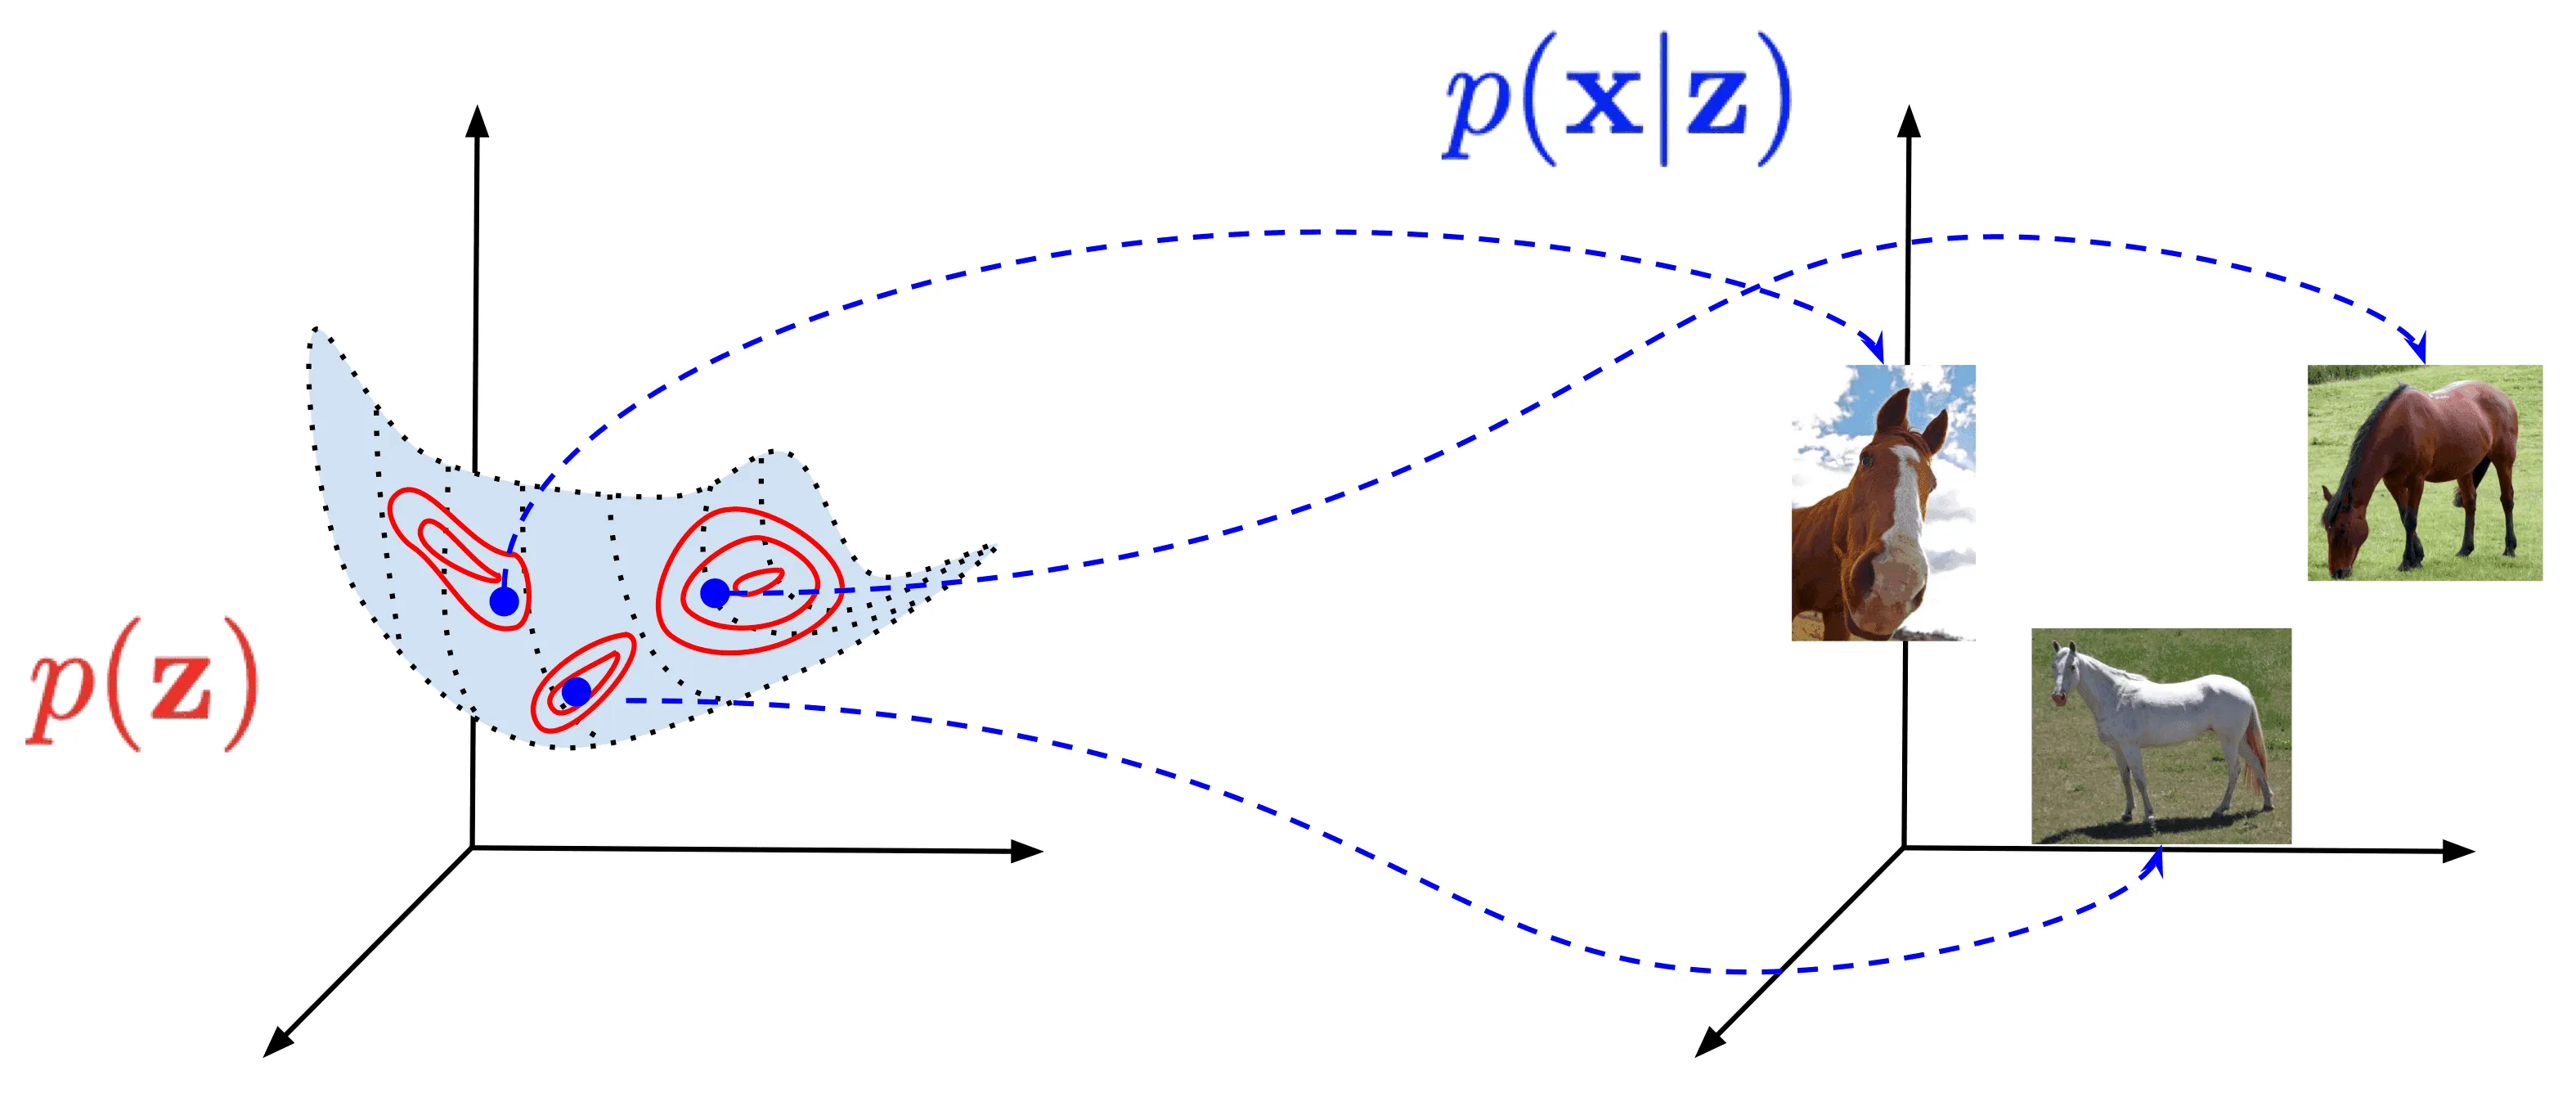
\includegraphics[width=.8\textwidth]{../resources/vae/sampling.png}
    \end{figure}
\end{frame}

\begin{frame}[allowframebreaks]{Интуиция}
    \textbf{Идея:}
    \begin{itemize}
        \item $f_{\boldsymbol{\theta}}(\boldsymbol{x}) = \boldsymbol{\psi}_{\boldsymbol{x}} = \left(\boldsymbol{\mu}_{\boldsymbol{x}}, \boldsymbol{\sigma}_{\boldsymbol{x}}^2\right)$ — параметры нормального распределения.
        \item $\boldsymbol{z} \sim p(\boldsymbol{z} \mid \boldsymbol{\psi}_{\boldsymbol{x}}) = \mathcal{N}(\boldsymbol{z} \mid \boldsymbol{\mu}_{\boldsymbol{x}}, \boldsymbol{\sigma}_{\boldsymbol{x}}^2)$.
        \item $\tilde{\boldsymbol{x}} = g_{\boldsymbol{\phi}}(\boldsymbol{z}) \sim p(\boldsymbol{x} \mid \boldsymbol{z})$.
    \end{itemize}

    \textbf{Параметры:}
    \begin{align*}
        \boldsymbol{\mu}_{\boldsymbol{x}}      & = \begin{bmatrix} \mu_{\boldsymbol{x}1} & \mu_{\boldsymbol{x}2} & \ldots & \mu_{\boldsymbol{x}M} \end{bmatrix},                                                \\
        \boldsymbol{\sigma}_{\boldsymbol{x}}^2 & = \operatorname{diag}\left(\begin{bmatrix} \sigma_{\boldsymbol{x}1}^2 & \sigma_{\boldsymbol{x}2}^2 & \ldots & \sigma_{\boldsymbol{x}M}^2 \end{bmatrix}\right).
    \end{align*}

    \framebreak

    \textbf{Проблемы:}
    \begin{enumerate}
        \item \textbf{Проблема 1:} модель стремится к $\boldsymbol{\sigma}_{\boldsymbol{x}}^2 = \mathbf{0}$, что превращает VAE в AE.
              \begin{itemize}
                  \item \textbf{Решение:} добавить регуляризационный член (какой?):
                        \begin{equation*}
                            \mathcal{L}(\boldsymbol{\theta}, \boldsymbol{\phi}) = \text{L}_{\text{rec}} + \alpha \text{L}_{\text{reg}}.
                        \end{equation*}
              \end{itemize}
        \item \textbf{Проблема 2:} сэмплирование не дифференцируемо.
    \end{enumerate}
\end{frame}

\begin{frame}{Правдоподобие $p(\boldsymbol{x})$}
    \textbf{Совместное распределение:}
    \begin{equation*}
        p_{\phi}(\boldsymbol{x}, \boldsymbol{z}) = p(\boldsymbol{x}, \boldsymbol{z} \mid \phi).
    \end{equation*}

    \textbf{Правдоподобие данных:}
    \begin{align*}
         & L(\phi) = \prod_{i=1}^N p_{\phi}(\boldsymbol{x}_i),          \\
         & \log L(\phi) = \sum_{i=1}^N \log p_{\phi}(\boldsymbol{x}_i).
    \end{align*}

    \textbf{Цель:} Максимизация правдоподобия:
    \begin{equation*}
        p_{\phi}(\boldsymbol{x}) = \int_{\boldsymbol{z}} p_{\phi}(\boldsymbol{x}, \boldsymbol{z}) d\boldsymbol{z} \to \max_{\phi \in \Phi}.
    \end{equation*}
\end{frame}

\begin{frame}[allowframebreaks]{Аппроксимация $p(\boldsymbol{z} \mid \boldsymbol{x})$}
    \textbf{Теорема Байеса:}
    \begin{equation*}
        p(\boldsymbol{z} \mid \boldsymbol{x}) = \frac{p(\boldsymbol{x}, \boldsymbol{z})}{p(\boldsymbol{x})} = \frac{p(\boldsymbol{x} \mid \boldsymbol{z}) p(\boldsymbol{z})}{p(\boldsymbol{x})}.
    \end{equation*}

    \textbf{Распределения:}
    \begin{itemize}
        \item $p(\boldsymbol{x})$: априорное распределение данных.
        \item $p(\boldsymbol{z} \mid \boldsymbol{x})$: распределение энкодера.
        \item $p(\boldsymbol{z}) = \mathcal{N}(\boldsymbol{z} \mid \mathbf{0}, \mathbf{E})$: априорное распределение латентного пространства.
        \item $p(\boldsymbol{x} \mid \boldsymbol{z}) \left(= \mathcal{N}(\boldsymbol{x} \mid g_{\boldsymbol{\phi}}(\boldsymbol{z}), c\mathbf{I})\right)$: распределение декодера.
    \end{itemize}

    \framebreak

    \textbf{Проблема:} $p(\boldsymbol{z} \mid \boldsymbol{x})$ имеет сложную форму:
    \begin{equation*}
        p(\boldsymbol{z} \mid \boldsymbol{x}) = \frac{\mathcal{N}(\boldsymbol{x} \mid g_{\boldsymbol{\phi}}(\boldsymbol{z}), c\mathbf{I}) \mathcal{N}(\boldsymbol{z} \mid \mathbf{0}, \mathbf{E})}{p(\boldsymbol{x})}.
    \end{equation*}

    \textbf{Workaround:} Аппроксимация через простое распределение $q(\boldsymbol{z})$:
    \begin{equation*}
        p(\boldsymbol{z} \mid \boldsymbol{x}) \approx q(\boldsymbol{z}) = \mathcal{N}(\boldsymbol{z} \mid \boldsymbol{\mu}_{\boldsymbol{x}}, \boldsymbol{\sigma}_{\boldsymbol{x}}^2).
    \end{equation*}
\end{frame}

\begin{frame}[allowframebreaks]{Вариационное приближение}
    \textbf{Цель:} Максимизировать правдоподобие $p(\boldsymbol{x})$:
    \begin{align*}
        \log p(\boldsymbol{x}) & = \log \int_{\boldsymbol{z}} p(\boldsymbol{x}, \boldsymbol{z})d\boldsymbol{z}  = \log \int_{\boldsymbol{z}} p(\boldsymbol{x} \mid \boldsymbol{z})p(\boldsymbol{z})d\boldsymbol{z} \\
                               & = \log \mathbb{E}_{q(\boldsymbol{z})}\left[\frac{p(\boldsymbol{z})p(\boldsymbol{x} \mid \boldsymbol{z})}{q(\boldsymbol{z})}\right].
    \end{align*}

    \textbf{Неравенства Йенсена:}
    \begin{align*}
         & g(\mathbb{E}[\xi]) \leq \mathbb{E}[g(\xi)], \quad g(x) \text{ \textemdash{} вогнутая функция}, \\
         & g(\mathbb{E}[\xi]) \geq \mathbb{E}[g(\xi)], \quad g(x) \text{ \textemdash{} выпуклая функция}.
    \end{align*}
    Применим к $\log$:
    \begin{align*}
        \log p(\boldsymbol{x}) & = \log \mathbb{E}_{q(\boldsymbol{z})}\left[\frac{p(\boldsymbol{z})p(\boldsymbol{x} \mid \boldsymbol{z})}{q(\boldsymbol{z})}\right] \geq \mathbb{E}_{q(\boldsymbol{z})}\left[\log \frac{p(\boldsymbol{z})p(\boldsymbol{x} \mid \boldsymbol{z})}{q(\boldsymbol{z})}\right] \\
                               & = \mathbb{E}_{q(\boldsymbol{z})}\left[\log p(\boldsymbol{x} \mid \boldsymbol{z})\right] - \mathbb{E}_{q(\boldsymbol{z})}\left[\log \frac{q(\boldsymbol{z})}{p(\boldsymbol{z})}\right]                                                                                    \\
                               & = \mathbb{E}_{q(\boldsymbol{z})}\left[\log p(\boldsymbol{x} \mid \boldsymbol{z})\right] - \text{KL}(q(\boldsymbol{z}) \parallel p(\boldsymbol{z})),
    \end{align*}
    где $\text{KL}$ — дивергенция Кульбака-Лейблера.

    \textbf{Итог:} Нижняя граница на $\log p(\boldsymbol{x})$ (Evidence Lower Bound, \textit{ELBO}):
    \begin{align*}
        \log p(\boldsymbol{x}) \geq \mathbb{E}_{q(\boldsymbol{z})}\left[\log p(\boldsymbol{x} \mid \boldsymbol{z})\right] - \text{KL}(q(\boldsymbol{z}) \parallel p(\boldsymbol{z})) \to \max_{q(\boldsymbol{z})}.
    \end{align*}
\end{frame}

\begin{frame}{Распределение $p(\boldsymbol{x} \mid \boldsymbol{z})$}
    $p(\boldsymbol{x} \mid \boldsymbol{z}) = \mathcal{N}(\boldsymbol{x} \mid g_{\boldsymbol{\phi}}(\boldsymbol{z}), c\mathbf{I})$, $c \neq 0$, поэтому матрица ковариации невырождена.

    \begin{align*}
        p(\boldsymbol{x} \mid \boldsymbol{z})
         & = \frac{1}{(2\pi)^{D/2}|c\mathbf{I}|^{1/2}}\exp\left(-\frac{1}{2}(\boldsymbol{x} - g_{\boldsymbol{\phi}}(\boldsymbol{z}))^T(c\mathbf{I})^{-1}(\boldsymbol{x} - g_{\boldsymbol{\phi}}(\boldsymbol{z}))\right) \\
         & = \frac{1}{(2\pi)^{D/2}c^{D/2}}\exp\left(-\frac{1}{2c}\|\boldsymbol{x} - g_{\boldsymbol{\phi}}(\boldsymbol{z})\|^2_2\right)                                                                                  \\
         \\
        \log(p(\boldsymbol{x} \mid \boldsymbol{z}))
         & = -\frac{D}{2}\log(2\pi) - \frac{D}{2}\log(c) - \frac{1}{2c}\|\boldsymbol{x} - g_{\boldsymbol{\phi}}(\boldsymbol{z})\|^2_2                                                                                   \\
         & = \text{const} - \frac{1}{2c}\|\boldsymbol{x} - g_{\boldsymbol{\phi}}(\boldsymbol{z})\|^2_2.
    \end{align*}
\end{frame}

\begin{frame}{Итоговая оптимизация}
    \textbf{Оптимизационная задача:}
    \begin{align*}
         & \mathbb{E}_{q(\boldsymbol{z})}\left[\log p(\boldsymbol{x} \mid \boldsymbol{z})\right] - \text{KL}(q(\boldsymbol{z}) \parallel p(\boldsymbol{z}))                                                                  \\
         & = -\mathbb{E}_{q(\boldsymbol{z})}\left[\frac{1}{2c}\|\boldsymbol{x} - g_{\boldsymbol{\phi}}(\boldsymbol{z})\|^2_2\right] - \text{KL}(q(\boldsymbol{z}) \parallel p(\boldsymbol{z})) \to \max_{q(\boldsymbol{z})}.
    \end{align*}

    \textbf{Эквивалентная формулировка:}
    \begin{align*}
         & \mathbb{E}_{q(\boldsymbol{z})}\left[\frac{1}{2c}\|\boldsymbol{x} - g_{\boldsymbol{\phi}}(\boldsymbol{z})\|^2_2\right] + \text{KL}(q(\boldsymbol{z}) \parallel p(\boldsymbol{z})) \to \min_{q(\boldsymbol{z})}.
    \end{align*}
\end{frame}

\begin{frame}{Вспомним интуицию}
    \textbf{Получили то, чего и хотели:}
    \begin{align*}
        \text{L}_{\text{rec}} & = \frac{1}{2c}\|\boldsymbol{x} - g_{\boldsymbol{\phi}}(\boldsymbol{z})\|^2_2, \\
        \text{L}_{\text{reg}} & = \text{KL}(q(\boldsymbol{z}) \parallel p(\boldsymbol{z})).
    \end{align*}

    \textbf{Итог:}
    Баланс между реконструкцией данных и отклонением от априорного распределения в латентном пространстве.
\end{frame}

\begin{frame}[allowframebreaks]{Вычисление $\text{L}_{\text{reg}}$}
    \begin{align*}
        & \text{KL}(q(\boldsymbol{z}) \parallel p(\boldsymbol{z})) = \text{KL}\left(\boldsymbol{\mathcal{N}}(\boldsymbol{z} \mid \boldsymbol{\mu}_{\boldsymbol{x}}, \boldsymbol{\sigma}_{\boldsymbol{x}}^2) \parallel \boldsymbol{\mathcal{N}}(\boldsymbol{z} \mid \mathbf{0}, \mathbf{E})\right) \\
        &= \text{KL}\left(\prod_{i=1}^M\boldsymbol{\mathcal{N}}(z_i \mid \mu_{\boldsymbol{x}i}, \sigma_{\boldsymbol{x}i}^2) \parallel \prod_{i=1}^M\boldsymbol{\mathcal{N}}(z_i \mid 0, 1)\right) = \text{KL}\left(\prod_{i=1}^Mq_i(\boldsymbol{z}_i) \parallel \prod_{i=1}^Mp_i(\boldsymbol{z}_i)\right) \\
        &= \int_{\boldsymbol{z}} \prod_{i=1}^Mq_i(\boldsymbol{z}_i)\log\frac{\prod_{i=1}^Mq_i(\boldsymbol{z}_i)}{\prod_{i=1}^Mp_i(\boldsymbol{z}_i)}d\boldsymbol{z} = \int_{\boldsymbol{z}} \prod_{i=1}^Mq_i(\boldsymbol{z}_i)\left(\sum_{i=1}^M\log \frac{q_i(\boldsymbol{z}_i)}{p_i(\boldsymbol{z}_i)}\right)d\boldsymbol{z} \\
        &= \sum_{j=1}^M\int_{\boldsymbol{z}} \log \frac{q_j(\boldsymbol{z}_j)}{p_j(\boldsymbol{z}_j)} \prod_{i=1}^Mq_i(\boldsymbol{z}_i) d\boldsymbol{z}_1\ldots d\boldsymbol{z}_M \\
        &= \sum_{j=1}^M \left( \left( \int_{\boldsymbol{z}_j} \log \frac{q_j(\boldsymbol{z}_j)}{p_j(\boldsymbol{z}_j)}q_j(\boldsymbol{z}_j) d\boldsymbol{z}_j \right) \prod_{i\neq j}^M \int_{\boldsymbol{z}_i} q_i(\boldsymbol{z}_i) d\boldsymbol{z}_i \right) = \ldots
    \end{align*}

    \begin{align*}
        &= \sum_{j=1}^M \left( \int_{\boldsymbol{z}_j} \log \frac{q_j(\boldsymbol{z}_j)}{p_j(\boldsymbol{z}_j)}q_j(\boldsymbol{z}_j) d\boldsymbol{z}_j \right) = \sum_{j=1}^M \text{KL}(q_j(\boldsymbol{z}_j) \parallel p_j(\boldsymbol{z}_j))
    \end{align*}

    \textbf{Для каждой компоненты:}
    \begin{align*}
        \text{KL}(q_j(\boldsymbol{z}_j) \parallel p_j(\boldsymbol{z}_j)) &= \int_{z_j} \mathcal{N}(z_j \mid \mu_{\boldsymbol{x}j}, \sigma_{\boldsymbol{x}j}^2) \log \frac{\mathcal{N}(z_j \mid \mu_{\boldsymbol{x}j}, \sigma_{\boldsymbol{x}j}^2)}{\mathcal{N}(z_j \mid 0, 1)} dz_j.\\
        &= \mathbb{E}_{q_j(z_j)}\left[\log \mathcal{N}(z_j \mid \mu_{\boldsymbol{x}j}, \sigma_{\boldsymbol{x}j}^2) - \log \mathcal{N}(z_j \mid 0, 1)\right].
    \end{align*}

    \textbf{Распределение $\mathcal{N}$:}
    \begin{align*}
        \log \mathcal{N}(z_j \mid \mu_{\boldsymbol{x}j}, \sigma_{\boldsymbol{x}j}^2) &= -\frac{1}{2}\log(2\pi\sigma_{\boldsymbol{x}j}^2) - \frac{1}{2\sigma_{\boldsymbol{x}j}^2}(z_j - \mu_{\boldsymbol{x}j})^2, \\
        \log \mathcal{N}(z_j \mid 0, 1) &= -\frac{1}{2}\log(2\pi) - \frac{1}{2}z_j^2.
    \end{align*}
    \textbf{Разница логарифмов:}
    \begin{align*}
        \log \mathcal{N}(z_j \mid \mu_{\boldsymbol{x}j}, \sigma_{\boldsymbol{x}j}^2) - \log \mathcal{N}(z_j \mid 0, 1) &= -\frac{1}{2}\log(\sigma_{\boldsymbol{x}j}^2) - \frac{1}{2\sigma_{\boldsymbol{x}j}^2}(z_j - \mu_{\boldsymbol{x}j})^2 + \frac{1}{2}z_j^2.
    \end{align*}

    \textbf{Итоговая формула:}
    \begin{align*}
        & \text{KL}(q_j(\boldsymbol{z}_j) \parallel p_j(\boldsymbol{z}_j)) = \mathbb{E}_{q_j(z_j)}\left[-\frac{1}{2}\log(\sigma_{\boldsymbol{x}j}^2) - \frac{1}{2\sigma_{\boldsymbol{x}j}^2}(z_j - \mu_{\boldsymbol{x}j})^2 + \frac{1}{2}z_j^2\right] \\
        &= \mathbb{E}_{q_j(z_j)}\left[ -\left(\frac{1}{2}\log(\sigma_{\boldsymbol{x}j}^2) + \frac{\mu_{\boldsymbol{x}j}^2}{2\sigma_{\boldsymbol{x}j}^2} \right) + \left(\frac{1}{2} - \frac{1}{2\sigma_{\boldsymbol{x}j}^2}\right)z_j^2 + \frac{\mu_{\boldsymbol{x}j}}{\sigma_{\boldsymbol{x}j}^2}z_j \right] \\
        &= -\left(\frac{1}{2}\log(\sigma_{\boldsymbol{x}j}^2) + \frac{\mu_{\boldsymbol{x}j}^2}{2\sigma_{\boldsymbol{x}j}^2} \right) + \left(\frac{1}{2} - \frac{1}{2\sigma_{\boldsymbol{x}j}^2}\right)\mathbb{E}_{q_j(z_j)}\left[z_j^2 \right] + \frac{\mu_{\boldsymbol{x}j}}{\sigma_{\boldsymbol{x}j}^2} \mathbb{E}_{q_j(z_j)}\left[z_j \right] = \ldots
    \end{align*}

    \textbf{Математические ожидания:}
    \begin{align*}
        & \mathbb{E}_{q_j(z_j)}\left[z_j \right] = \mu_{\boldsymbol{x}j}, \\
        & \mathbb{D}_{q_j(z_j)}\left[z_j \right] = \mathbb{E}_{q_j(z_j)}\left[z_j^2 \right] - \mu_{\boldsymbol{x}j}^2 = \sigma_{\boldsymbol{x}j}^2 \quad\Rightarrow\quad\mathbb{E}_{q_j(z_j)}\left[z_j^2 \right] = \sigma_{\boldsymbol{x}j}^2 + \mu_{\boldsymbol{x}j}^2.
    \end{align*}
    \textbf{Подстановка:}
    \begin{align*}
        \ldots 
        &= -\frac{1}{2}\log(\sigma_{\boldsymbol{x}j}^2) - \frac{\mu_{\boldsymbol{x}j}^2}{2\sigma_{\boldsymbol{x}j}^2} + \frac{1}{2}\left(1 - \frac{1}{\sigma_{\boldsymbol{x}j}^2}\right)(\sigma_{\boldsymbol{x}j}^2 + \mu_{\boldsymbol{x}j}^2) + \frac{\mu_{\boldsymbol{x}j}}{\sigma_{\boldsymbol{x}j}^2} \mu_{\boldsymbol{x}j} \\
        &= -\frac{1}{2}\log(\sigma_{\boldsymbol{x}j}^2) - \frac{\mu_{\boldsymbol{x}j}^2}{2\sigma_{\boldsymbol{x}j}^2} + \frac{1}{2}\left(\sigma_{\boldsymbol{x}j}^2 + \mu_{\boldsymbol{x}j}^2 - 1 - \frac{\mu_{\boldsymbol{x}j}^2}{\sigma_{\boldsymbol{x}j}^2} \right) + \frac{\mu_{\boldsymbol{x}j}^2}{\sigma_{\boldsymbol{x}j}^2} \\
        &= -\frac{1}{2}\log(\sigma_{\boldsymbol{x}j}^2) + \frac{1}{2}\sigma_{\boldsymbol{x}j}^2 + \frac{1}{2}\mu_{\boldsymbol{x}j}^2 - \frac{1}{2} \\
        &= \frac{1}{2}\left( \sigma_{\boldsymbol{x}j}^2 + \mu_{\boldsymbol{x}j}^2 - 1 - \log(\sigma_{\boldsymbol{x}j}^2) \right)
    \end{align*}
\end{frame}

\begin{frame}{Функционал потерь}
    \textbf{Итоговые формулы:}
    \begin{align*}
        \text{L}_{\text{rec}} &= \frac{1}{2c}\|\boldsymbol{x} - g_{\boldsymbol{\phi}}(\boldsymbol{z})\|^2_2, \\
        \text{L}_{\text{reg}} &= \sum_{j=1}^M \frac{1}{2}\left( \sigma_{\boldsymbol{x}j}^2 + \mu_{\boldsymbol{x}j}^2 - 1 - \log(\sigma_{\boldsymbol{x}j}^2) \right).
    \end{align*}
    \textbf{Дополнение:} Для $\text{L}_{\text{rec}}$ также можно использовать кросс-энтропию.
\end{frame}

\begin{frame}{Reparametrization trick}
    \begin{align*}
        \boldsymbol{z}_j &\sim \boldsymbol{\mathcal{N}}( \boldsymbol{z}_j \mid \mu_{\boldsymbol{x}j}, \sigma_{\boldsymbol{x}j}^2) \Leftrightarrow
        \begin{cases}
            & \boldsymbol{\varepsilon}_j \sim \boldsymbol{\mathcal{N}}(0, 1), \\
            & \boldsymbol{z}_j = \mu_{\boldsymbol{x}j} + \sigma_{\boldsymbol{x}j}\boldsymbol{\varepsilon}_j.
        \end{cases}
    \end{align*}

    \textbf{Поскольку:}
    \begin{align*}
        p_{\varepsilon}(\varepsilon) &= \frac{1}{\sqrt{2\pi}}\exp\left(-\frac{\varepsilon^2}{2}\right), \\
        \varepsilon &= \frac{z - \mu_{\boldsymbol{x}}}{\sigma_{\boldsymbol{x}}}, \quad \sigma_{\boldsymbol{x}} > 0, \\
        \left|\frac{d\varepsilon}{dz}\right| &= \frac{1}{\sigma_{\boldsymbol{x}}}, \\
        p_z(z) &= p_{\varepsilon}\left(\frac{z - \mu_{\boldsymbol{x}}}{\sigma_{\boldsymbol{x}}}\right)\left|\frac{d\varepsilon}{dz}\right| = \frac{1}{\sqrt{2\pi}\sigma_{\boldsymbol{x}}}\exp\left(-\frac{(z - \mu_{\boldsymbol{x}})^2}{2\sigma_{\boldsymbol{x}}^2}\right).
    \end{align*}
\end{frame}

\begin{frame}{Архитектура VAE}
    \begin{figure}
        \centering
        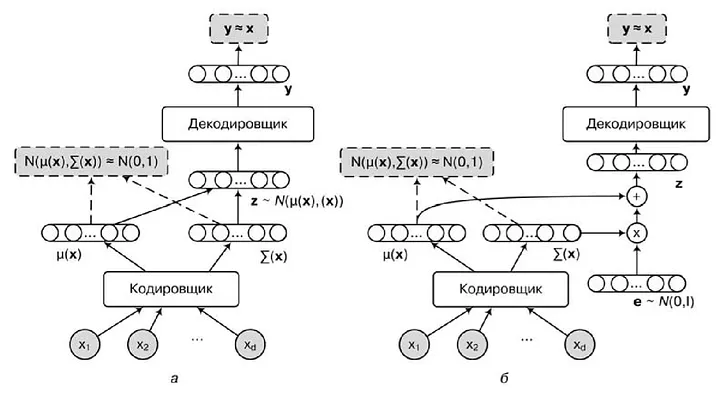
\includegraphics[width=1\textwidth]{../resources/vae/vae.png}
    \end{figure}
\end{frame}

\begin{frame}{Детали реализации}
    \textbf{Проблема:} $\forall i \quad 0 < \boldsymbol{\sigma}_{\boldsymbol{xi}}^2 \ll 1$ \textemdash{} маленькие значения могут приводить к ошибкам численных расчетов.

    \textbf{Решение:} Использовать логарифмированное значение $\boldsymbol{\sigma}_{\boldsymbol{xi}}^2$:
    \begin{equation*}
        \log \boldsymbol{\sigma}_{\boldsymbol{xi}}^2  \in \mathbb{R}^M.
    \end{equation*}

    \textbf{Репараметризация:}
    \begin{align*}
        \boldsymbol{\varepsilon}_j &\sim \boldsymbol{\mathcal{N}}(0, 1), \\
        \boldsymbol{z}_j &= \mu_{\boldsymbol{x}j} + \exp\left(\frac{1}{2}\log \boldsymbol{\sigma}_{\boldsymbol{xi}}^2 \right)\boldsymbol{\varepsilon}_j.
    \end{align*}
\end{frame}

\begin{frame}{Практика}
    \begin{figure}
        \centering
        
\includegraphics[width=.3\textwidth]{../resources/overall/Jupyter_logo.png}
    \end{figure}
\end{frame}

